\documentclass[a4paper, 12pt]{article}
% Allow the usage of graphics (.png, .jpg)
\usepackage[pdftex]{graphicx}
\graphicspath{ {./images/} }
\usepackage{apacite}
\usepackage[T1]{fontenc}
\usepackage{url}
\usepackage{amsmath}

% set line spacing
\usepackage{setspace}
\setlength{\parindent}{0pt}
\setlength{\parskip}{2ex}
\linespread{1.3}

\usepackage{tocloft} % for list of equations
% define list of equations
\newcommand{\listequationsname}{\Large{List of Equations}}
\newlistof{myequations}{equ}{\listequationsname}
\newcommand{\myequations}[1]{
   \addcontentsline{equ}{myequations}{\protect\numberline{\theequation}#1}
}
\setlength{\cftmyequationsnumwidth}{2.3em}
\setlength{\cftmyequationsindent}{1.5em}

% Comment the following line to NOT allow the usage of umlauts
\usepackage[utf8]{inputenc}
%custom margins
\usepackage[]{vmargin}
\setpapersize{A4}	
\setmarginsrb{35mm}{30mm}{30mm}{20mm}{0pt}{0mm}{12pt}{13mm}
% Correct hyphenation in urls
\usepackage{url}
% Support long tables
\usepackage[]{longtable}
\usepackage{ltablex}
\usepackage{adjustbox}
%Pretty bibliography in UEF format
\usepackage{natbib}
% verbatim code listings
\usepackage{listings}
%Unobtrusive in document links
\usepackage{hyperref}
\hypersetup{
    colorlinks,
    citecolor=black,
    filecolor=black,
    linkcolor=black,
    urlcolor=black
}

\begin{document}

\pagenumbering{gobble}

% do cover pages
%Fill these in and they'll propagate across the title page. Remember to keep the space at the end!
\def \ajankohtaenglish {July 2021 }
\def \authorname {Hiep Nguyen }
\def \thesistitle {Trajectory Clustering }
\def \campus {Joensuu }
\def \facultyschooleng {School of Computer Science }
%FT = PhD, FM = MSc
\def \supervisorseng {Pasi Fr{\"a}nti and Radu Mariescu-Istodor}

\def \documenttypeeng {Master's Thesis }
%\def \documenttypeeng {Bachelor's Thesis}

%Number of non-cover pages, to last page of references
\def \mypagecount {70 }

\graphicspath{ {./images/} }

%%%%%%%%%%%%%%%%%% TITLE PAGE %%%%%%%%%%%%%%%%%%

\vspace*{3cm}
\vspace{0.5cm}

\begin{center}
\begin{LARGE}\thesistitle \end{LARGE}

\vspace{1.5cm}

\begin{Large}\authorname \end{Large}

\vspace{\stretch{1}}

{\large
\documenttypeeng
~\\
% to have it in black and white, swap the commented line
% \includegraphics[width=7cm]{UEF_fin_pysty_1_cmyk}\\
\includegraphics[width=7cm]{UEF logo.png}\\
Faculty of Science and Forestry\\
\facultyschooleng \\
\ajankohtaenglish \\
}
\end{center}

\vspace{0.5cm}

\thispagestyle{empty}

\begin{spacing}{1.0}
\newpage

%%%%%%%%%%%%%%%%%% Abstract page in English %%%%%%%%%%%%%%%%%%

UNIVERSITY OF EASTERN FINLAND, \\ Faculty of Science and Forestry, \campus \\ School of Computing \\
\facultyschooleng \\ \\
Student, \authorname : \thesistitle \\
\documenttypeeng , \mypagecount p.
Supervisors of the \documenttypeeng : \supervisorseng \\
\ajankohtaenglish \\

Abstract: In the past few years, there has been a significant advancement in the development of location-based positioning devices, and an increasing number of moving objects and their trajectories are being captured. Thus, it follows that the subject of moving object trajectory clustering is certain to be of prime importance to researchers working on data mining on moving objects. To give a context, we look at how development and the current trend in moving object clustering are in and then review common clustering techniques presented in the past few years.  In this thesis, we start by summarizing the basic characteristics of a trajectory. Second, we examine the metrics for determining the similarity/dissimilarity of two trajectories. Thirdly, we investigate the methods and implementation processes of conventional moving object clustering methods. Finally, the validation criteria used to assess the efficacy and efficiency of clustering algorithms are explored. 

% Key words English

~\\ % Tämä tekee tyhjän rivin; älä editoi tätä pois
Keywords:
trajectory, distance, similarity, clustering

% CR-luokat

% ACM-luokitus löytyy Computing Reviews -lehden jokaisen
% vuosikerran ensimmäisestä numerosta sekä verkosta
% osoitteesta http://www.acm.org/class/

% Ota omat luokkasi tuoreimmasta vuosikerrasta.

CR Categories (ACM Computing Classification System,
1998 version): A.m, K.3.2\\

\end{spacing}

\newpage

%%%%%%%%%%%%%%%%%% Foreword/Preface %%%%%%%%%%%%%%%%%%

\section*{Foreword}
I am grateful to the University of Eastern Finland and to all of the teachers who helped me to obtain knowledge in many fields of computer science. It was a good opportunity for me to participate in the IMPIT programme. 

I would like to thank my thesis supervisors, Professor Pasi Fr{\"a}nti and Dr. Radu Mariescu-Istodor, for their guidance throughout the years. I would not have been able to finish my thesis without their dedications, valuable suggestions, and advise. I believe that my research and time management have been improved significantly through their instructions.

In the end, I want to express my appreciation and love to my family and friends for their mental support and encouragement.

\newpage

%%%%%%%%%%%%%%%%%% Abbrieviations %%%%%%%%%%%%%%%%%%

\section*{List of Abbreviations}

\begin{tabular}{lp{12.5cm}}

C-SIM & Cell-based similarity \\

CI & Centroid Index \\

CSI & Centroid Similarity Index \\

DBSCAN & Density-based spatial clustering of applications with noise \\

DTW & Dynamic Time Warping \\

GPS & Global Positioning System \\

HC-SIM & Hierarchical Cell Similarity \\

HCA & Hierarchical Cluster Analysis \\

LCSS & Longest Common Subsequence \\

PSI & Pair Sets Index \\

SSE & Sum of squares error \\

SSB & Sum of squares between the clusters \\

SSW & Sum of squares within the clusters

\end{tabular}

\newpage

% ----------------- Table of Contents -------------

\setlength{\parskip}{0ex}

\tableofcontents
\newpage

\listoftables
\newpage

\listoffigures
\newpage

\listofmyequations
\newpage

\setlength{\parskip}{2ex}

\tableofcontents

\listoftables

\listoffigures

\listofmyequations

\cleardoublepage

\begin{abstract} 
In the past few years, there has been a significant advancement in the development of location-based positioning devices, and an increasing number of moving objects and their trajectories are being captured. Thus, it follows that the subject of moving object trajectory clustering is certain to be of prime importance to researchers working on data mining on moving objects. To give a context, we look at how development and the current trend in moving object clustering are in and then review common cluster techniques presented in the past few years.  In this thesis, we start by summarizing the basic characteristics of trajectory. Second, we examine the metrics for determining the similarity/dissimilarity of two trajectories. Thirdly, we investigate the methods and implementation processes of conventional moving object clustering methods. Finally, the validation criteria used to assess the efficacy and efficiency of clustering algorithms are explored. 
\end{abstract}

\pagebreak

\pagenumbering{arabic} % arabic(1234) numbering, autoreset to 1

\section{Introduction}
The increasing usage of integrated mobile devices integrate with GPS, WI-FI, and data storage hardware allow us to gather a massive quantity of data. Due to the intricacy of the collected data, extract useful information is a challenging problem to solve. Knowing principal routes that people or vehicles follow during the day can provide valuable information for the analysis of mobility. For instance, the presence of important routes not adequately covered by the public transport service could be highlighted by a set of trajectories, which provide information on how to improve it. Trajectory clustering is an appropriate way of analyzing trajectory data and has been applied to road network extraction \citep{mariescu2018cellnet}, \citep{ahmed2015comparison} and \citep{biagioni2012inferring}, detecting taxi fraud \citep{liu2013fraud}, data compression \citep{chen2012compression}, etc. Additionally, trajectory clustering is used to gather temporal-spatial information in the trajectory data and is widely used in many application areas, such as motion prediction \citep{chen2010searching} and traffic monitoring \citep{atev2006learning}

Trajectory data is stored in a variety of forms based on the kind of device, the velocity of the object, and even the function. For instance, a GPS device generates a trajectory, which is a locations sequence in a geographical space identified by a combination of coordinates and a time stamp. Additional object-related attributes such as direction, velocity, or geographic information may be added in certain cases \citep{ying2011semantic, ying2010mining}. Multidimensional data is used in different areas, for example, to better understand animal migratory patterns by examining animal trajectories, to help forecast the weather by analyzing hurricane data, to help athletes achieve higher levels of performance, and much more.  

\begin{figure}[ht]
    \centering
    \includegraphics[width=0.75\textwidth]{Trajectories.png}
    \caption{Trajectories with varying lengths}
    \label{fig1}
\end{figure}

Measurement of how similar two trajectories are is a typical approach in a wide range of applications. As a result, the measurement of distances is necessary for many tasks and applications of trajectory analysis since it enables us to judge the similarity of two trajectories. The spacing between the trajectories must be properly determined. Because trajectories are high-dimensional data (a sequence of positions on a map/a time-series of positions on a time-line) that has both spatial and temporal qualities, they must be taken into consideration when doing calculations like distance measurements. Therefore, there are several distance metrics used for trajectory data. E.g., the term "measure the sequence-only distance between trajectories" may include concepts such as Euclidean distance and Dynamic Time Wrapping Distance (DTW). Various approaches, including clustering and classification, are often employed to identify valuable patterns from large volumes of trajectory data. Clustering is an unsupervised learning method that organizes data based on their distance \citep{han2011data,xu2005survey}. Trajectories that occur in each cluster tend to be rather similar and distinct from those in other clusters \citep{berkhin2006survey,besse2015review, yuan2017review}.

\begin{figure}[ht]
    \centering
    \includegraphics[width=1\textwidth]{Cluster Methods.png}
    \caption{Clustering Methods}
    \label{fig2}
\end{figure}

There are two primary methodologies used for data clustering like trajectories. Specify trajectory clustering algorithms first, then use generic clustering methods to compare trajectory distance/dissimilarity. Density-based clustering \citep{kriegel2011density} is one of the most ideal clustering methods for trajectories since it can extract clusters of any form and is also tolerant to outliers \citep{ester1996density}. Density-Based Spatial Clustering of Applications with Noise (DBSCAN), is one of the most extensively used approaches in this group, which is commonly used \citep{zhao2019trajectory,cheng2018density,chen2011clustering,lee2007trajectory}. Fundamental to the clustering challenge is measuring similarity. To measure similarity (inverse distance), it should be done before grouping. The definition of distance in spatial trajectories is significantly complicated. Trajectories are non-linear sequences of points with various lengths in multiple dimensions. Thus, to compare two trajectories, a comprehensive approach is required to fully determine the distance between them. Different distance metrics are presented according to the analysis's goal and the data type. Due to the domain-specific nature of the concept of similarity, distinct distance metrics are defined to address various aspects of similarity, are temporal, spatio-temporal, and spatial. Euclidean, Fréchet, Hausdorff, DTW, and LCSS distances are the fundamental metrics in measuring similarity from which many additional metrics are derived \citep{abbaspour2017method,aghabozorgi2015time,wang2013effectiveness}.

\section{Model for trajectory clustering}
A trajectory is a series of time-stamped data that captures the path of moving things, such as humans, cars, animals, and natural features. For example, Global Position System (GPS) tracking devices generating a trajectory as $Trajectory=(A,B,\cdots,T_{n})$, which is a consecutive spatial space sequence of points, and $T_{i}$ indicates a combination of coordinates and timestamps such as $T_i=(x_{i},y_{i},t_{i})$.

Clustering methods are designed to aggregate similar trajectories into distinct groups. This is a challenging task due to the trajectory complication, as objects within a particular region can take numerous paths. Clustering trajectories may be done in a variety of ways. We will focus on trajectory clustering based on distance but have also investigated alternative techniques. In most situations, trajectory data is represented as a multidimensional (2D or 3D) time series as in \autoref{fig3}; \cite{gaffney1999trajectory}, \cite{vasquez2004motion}. \cite{chen2012compression} used GPS trajectory clustering for improving data compression. The continuous definition of trajectory also applies by \cite{gariel2011trajectory} to re-sample trajectories to achieve equal-length time series. These new trajectories are then analyzed for the main components to obtain and finally cluster the primary components. The purpose is to group trajectories that follow similar paths. As clustering is focused on trajectories, and it necessitates a new distance measurement to define the similarity between them.

There has been considerable effort put into developing different trajectory distances. Numerous approaches have been employed to cluster trajectories from data collection. Clustering techniques based on Euclidean distance provide erroneous results since trajectories include a variable number of points. As a result, numerous warping distance-based techniques have been established. Typical examples are distance measurements based on Dynamic Time Warping (DTW), and Longest Common Subsequence (LCSS), all of which reorder trajectories' time index to obtain a perfect match. Another possibility is to concentrate on the shape of the trajectories. Hausdorff and Fréchet, for example, maybe adapted to trajectories. In the next section, we will study and compare several distances on the trajectory. 

\begin{figure}[ht]
    \centering
    \includegraphics[width=1\textwidth]{Trajectory.png}
    \caption{A GPS trajectory with 7076 points \citep{qian2017simplifying}.}
    \label{fig3}
\end{figure}

\pagebreak

\section{Trajectory Distance}
A trajectory distance generalization that considered moving objects and measures on average how close two objects were during some time period. $d(A,B)$ represents the distance of two trajectories $A\,and\,B$. The greater the value, the less similarity between the two trajectories. Apart from the concept of mathematical distance, several measurements may be utilized to characterize this dissimilarity. Distances may be classified into two types: those based on the geometry of the trajectory (Shape-based distances) and those that consider temporal dimension (Warping based distance). 

\subsection{Warping based distance}
In the 1960s, Euclidean distance was suggested to calculate distance between time series, and now, during the last several decades, has been recognized to be one of the most commonly used distance functions \citep{keogh2000scaling,faloutsos1994fast,pfeifer1980three,priestley1980state}.

\begin{figure}[ht]
    \centering
    \includegraphics[width=0.5\textwidth]{Euclidean.png}
    \caption{Euclidean distance}
    \label{fig4}
\end{figure}

The Euclidean distance $d_{Euclidean}(A, B)$ between trajectories $A\,and\,B$ with the same size $n$ is define as follows:
\begin{equation} \label{eq1}
    d_{Euclidean}(A, B) = \frac{\sum_{i=1}^n d(a_{i}, b_{i})}{n}
\end{equation}
\myequations{Euclidean distance}

Where $a_{i}$ and $b_{i}$ is the ith sample point of two trajectories $A$ and $B$. The time complexity of Euclidean distance is $O(n)$. 

The Euclidean distance measure is simple to understand; however, it is only accurate if the compared trajectories are of equal size, which is not likely to be the case in practical applications. The primary objective of warping distance is to resolve this issue. The dynamic time warping algorithm (DTW) \citep{kruskal1983overview} and the longest common subsequence algorithm (LCSS) \citep{kearney1990stream} were introduced to increase the accuracy. While both distances are specified identically, they use distinct cost functions.

\subsubsection{DTW}
\textit{Dynamic time warping} (DTW) is a similarity method for comparing two sequences. In the beginning, \cite{myers1980performance} developed DTW to calculate time-series distance. In the 1980s, DTW was introduced to measure trajectory distance \citep{kruskal1983overview} and has become one of the most extensive methods for measuring trajectory distance. DTW explores all point alignments between two trajectories in search of the distance which is minimum. 

\begin{figure}[ht]
    \centering
    \includegraphics[width=0.5\textwidth]{DTW.png}
    \caption{DTW distance}
    \label{fig5}
\end{figure}

Specifically, the DTW distance $d_{DTW} (A,B)$ between two trajectories $A$ and $B$ is defined as:
\begin{equation} \label{eq2}
    d_{DTW} (A,B) = \begin{cases}
                        0, if\:n\:=\:0\:and\:m\:=\:0 \\
                        \infty, if\:n\:=\:0\:or\:m\:=\:0 \\
                        d(Head(A), Head(B)) + min\{d_{DTW}(A, Rest(B)), \\ d_{DTW}(Rest(A), B), d_{DTW}(Rest(A), Rest(B) \} \: otherwise
                    \end{cases}
\end{equation}
\myequations{DTW distance}
With $Head(A)$ denotes $a_1$, $Rest(A)$ denotes $\{a_2, \dots, a_n\}$ in case trajectory $A$ is consists of GPS points $\{a_1, \dots, a_n\}$. $n$, $m$ are trajectories $A$ and $B$ lengths. DTW's time complexity is $O(mn)$.

\subsubsection{LCSS}
\textit{Longest common subsequence} (LCSS) is a well-known method for measuring string similarity that searches for the longest common sub-sequence between two strings. For example, for two sequences 'ABCD' and 'ACBAD', their longest sub-sequences are 'ABD' and 'ACD'. Because a trajectory may be considered as a series of sample points, LCSS was used to compare the similarity of trajectories. However, it is difficult to identify two sample points with identical geographical information. When comparing trajectories $A\,and\,B$, LCSS considers $a_{i}\,(a_{i} \in A)\,and\,b_{j}\,(b_{j} \in B)$ to be the same if their distance is less than a threshold $\epsilon$. Therefore, we will ignore some sample points of $A\,and\,B$ which are too far apart to contribute. 

\begin{figure}[ht]
    \centering
    \includegraphics[width=0.5\textwidth]{LCSS.png}
    \caption{LCSS}
    \label{fig6}
\end{figure}

In contrast to Euclidean distance, LCSS is robust to noise. LCSS similarity is defined as:
\begin{equation} \label{eq3}
    \operatorname s_{LCSS}(A, B)=\left\{\begin{array}{c}0, \text { if } n=0 \text { or } m=0 \\ 1+\operatorname{LCSS}(\operatorname{Rest}(A), \operatorname{Rest}(B)), \text { if } d(\operatorname{Head}(A), \operatorname{Head}(B)) \leq \varepsilon \\ \max (\operatorname{LCSS}(\operatorname{Rest}(A), B), \operatorname{LCSS}(A, \operatorname{Rest}(B))), \text { otherwise }\end{array}\right.
\end{equation}
\myequations{LCSS Similarity}

LCSS is similarity, so we will calculate the distance:
\begin{equation} \label{eq4}
    d_{LCSS}(A, B) = 1 - s_{LCSS}(A,B)
\end{equation}
\myequations{LCSS Distance}

\subsubsection{Pros and Cons}
DTW and LCSS enable to comparison of different length trajectories. 

However, there are two major drawbacks to using warping-based distance:
\begin{itemize}
    \item In general, warping methods compare sequences one-to-one so choosing a series as a reference for other sequences is necessary. Two sequences must be well-balanced in order to detect changes in time series such as when there was acceleration and deceleration. Therefore, the sequence to be referenced must be carefully selected.
    \item Due to the inherent noise in traffic data, traditional warping-based methods cannot obtain accurate results when examining time series.
\end{itemize}

\subsection{Shape based distance}
Instead of matching the trajectory sample points, these distances compare the shape of trajectories. This indicates that trajectories are clustered regardless of their location. The most well-known distances are the Hausdorff and Fréchet.

\subsubsection{Fréchet distance}
The Fréchet distance \citep{eiter1994computing} is a method that measure similarity between curves considers both the location and sequence of points. The Fréchet distance between the two curves is the shortest length of leash necessary for both paths to be traversed.

\begin{figure}[ht]
    \centering
    \includegraphics[width=0.5\textwidth]{Frechet.png}
    \caption{Fréchet distance}
    \label{fig7}
\end{figure}

The Fréchet distance algorithm is shown below:
\begin{equation} \label{eq5}
    d_{Frechet}(A,B) = infmax_{t in [t.start, t.end]} \{d(f_{a}(t), f_{b}(t))\}
\end{equation}
\myequations{Fréchet distance}

$f_{a}\,and\,f_{b}$ denote as two continuous functions of two trajectories $A\,and\,B$ over time $t$, $t.start$ and $t.end$ denote starting time and end time of time period $t$ respectively. The Fréchet distance between $A\,and\,B$ is defined as the infimum over all reparameterizations $f_{a}(t)$ and $f_{b}(t)$. Fréchet distance is affected by variations in sampling rate and is susceptible to noise since it is the longest distance between two trajectories at the same time.

Fréchet distance's time complexity is $O(mn)$. 

\subsubsection{Hausdorff distance}
The Hausdorff distance is a metric distance which calculates the distance between two subsets of a metric space. It is the maximum distances from a point in one set to the closest point in the other set.

The Hausdorff distance algorithm is shown as:
\begin{equation} \label{eq6}
    d_{Hausdorff}(A,B) = max \{ \sup_{a \in A} \inf_{b \in B} d(a, b), \sup_{b \in B} \inf_{a \in A} d(a, b) \}
\end{equation}
\myequations{Hausdorff distance}

\begin{figure}[ht]
    \centering
    \includegraphics[width=0.5\textwidth]{Hausdorff.png}
    \caption{Hausdorff distance}
    \label{fig8}
\end{figure}

The Hausdorff distance's time complexity is $O(n^2)$. 

\subsubsection{Pros and Cons}
Both the Fréchet and Hausdorff distances are metrics, which means they correspond to the triangle inequality. If we want the clustering methods like DBSCAN or K-medoid to be efficient, we need this property of the distance. They've been used in many areas where shape comparison is required. However, it may be difficult to do a comprehensive comparison of trajectories. Both distances return the greatest distance between two trajectories at particular moments.

\begin{figure}[ht]
    \centering
    \includegraphics[width=1\textwidth]{hausdorff_frechet_distance.png}
    \caption{Distances calculated by Hausdorff and Fréchet \citep{besse2015review}}
    \label{fig9}
\end{figure}

As in \autoref{fig9}, we can see that $T^1$ and $T^2$ are the most comparable of the three trajectories, yet they are the furthest apart in Fréchet due to the maximum distance of trajectory end at 6. And the Hausdorff distances for all trajectories are nearly identical, implying poor precision. These two approaches are effective in applications involving shape comparisons, such as image comparison. 

\subsection{HC-SIM}
\cite{franti2021averaging} proposed a new shape-based distance, HC-SIM (Hierarchical Cell Similarity), an independent variant of C-SIM measure. We will evaluate HC-SIM in this thesis and compare it with other distances. HC-SIM are proposed as it is least impacted by sample rate changes and works well with noise.

\pagebreak

\begin{figure}[htbp!]
    \centering
    \includegraphics[width=0.8\textwidth]{csim.png}
    \caption{C-SIM}
\end{figure}

C-SIM algorithm was proposed by \cite{mariescu2017grid} to compute the similarity of two trajectories. It computes a cell representation for the two trajectories using a grid and determines the proportion of cells that are in common with the total cells. 

\textbf{C-SIM}:

\begin{equation} \label{eq7}
    S\left(C_{\mathrm{A}}, C_{\mathrm{B}}\right)=\frac{\left|C_{\mathrm{A}} \cap C_{\mathrm{B}}\right|+\left|C_{\mathrm{A}} \cap C_{B}^{d}\right|+\left|C_{\mathrm{B}} \cap C_{A}^{d}\right|}{\left|C_{\mathrm{A}}\right|+\left|C_{\mathrm{B}}\right|+\left|C_{\mathrm{A}}\right|+\left|C_{\mathrm{A}} \cap C_{\mathrm{B}}\right|}
\end{equation}
\myequations{C-SIM}

The C-SIM time complexity is $O(N_A + N_B + |C_A| + |C_B|)$ where $N_A$ and $N_B$ are the number of trajectories' points.

HC-SIM implements a grid featuring six layers (0.5\%, 1\%, 2\%, 4\%, 8\%, and 16\%). At each layer, we calculate how many cells are shared by two segments to the total number of cells they occupy.  In this thesis, we calculate HC-SIM distance through dissimilarity measurements:

\begin{equation} \label{eq8}
    \text{HC-SIM}(A, B) = \frac{1}{L} \sum_{i=1}^{L}\text{C-SIM}(A, B)
\end{equation}
\myequations{HC-SIM}

\begin{equation} \label{eq9}
    d_\text{HC-SIM}(A, B) = 1 - \text{HC-SIM}(A, B)
\end{equation}
\myequations{HC-SIM distance}

\section{Clustering}
Clustering is the most common unsupervised learning method in pattern recognition. It is basically the task of grouping objects such that similar objects reside in the same group together. Clustering algorithms have gained a lot of attention among researchers and therefore, numerous clustering algorithms have been evolved. In order to be successful with clustering, we first need to understand the nature of the objects we need to cluster. We need to examine their properties and understand how these objects are inputted into an algorithm. For instance, one may be interested to know whether the data that needs to be clustered is inputted into the algorithm incrementally. This is an interesting problem when data is collected as clusters are evolving. On the other hand, the data set can be present as a whole prior to the execution of the clustering algorithm. Additionally, the properties of the objects that need to be clustered are very important. These properties can give rise to a number of important questions such as if the objects are vector-based or if the objects are metric-based. Moreover, one needs to know if objects can be transformed from one form to another so that further analysis can be done on them. One of the most important aspects of clustering is a way of comparing the objects which are widely known as a distance function. 

In this section, we will explore clustering algorithms and make an attempt to show which clustering algorithm is reasonable for trajectory clustering. We first start off with some prerequisites that many clustering algorithms require and show that these requirements are met by the trajectory distance function. 

\subsection{Methods}

% Clustering algorithms are generally designed to be able to target a large class of objects. However, some algorithms have specific assumptions on the type of objects that are to be clustered. The most general assumption is a mathematical definition for the objects so they can be stored in memory or on a storage device using a data structure. Perhaps the second most widely accepted requirement is a distance function so the algorithm would be able to say how similar two objects are relative to another. Clustering algorithms use a vector-based representation of the objects so each object can be represented as a point in a k-dimensional space and typically the Euclidean distance is used as the distance function between the points. Observe that such assumptions can be very strong in real world problems. We know that we have a mathematical representation of our trajectories. We have also discussed the distance function between the trajectories and we also know that the trajectory distance function follows the metric space rules: it is symmetrical, and it follows the triangulation property. HAC (Hierarchical Agglomerative Clustering) method only requires a distance function between the objects.

\subsubsection{K-means}

K-means is the well-known unsupervised machine learning technique for partitioning data set into k clusters, where k the is predefined number of clusters. It classifies objects into a number of clusters that objects in the same cluster are similar while objects from other clusters are dissimilar. K-means represents each cluster by its center (also known as the centroid) which matches the mean of data points.

The primary principle underlying k-means clustering is to define clusters that the sum of square errors (SSE) or total within-cluster variation is minimized. 

The K-means algorithm is summarized as follows:

\begin{itemize}
    \item Define the number of clusters (k).
    \item Randomly select k objects from the data set as the initial cluster centroids.
    \item Allocates each observation to the closest cluster.
    \item Compute the centroids for the clusters by calculating the mean of all data points that belong to each cluster.
    \item Loop through steps 3 and 4 until the cluster assignments stay unchanged.
\end{itemize}

K-means is a simple algorithm. By using a better initialization method and restarting k-means, it can be significantly enhanced \citep{franti2019much}. Furthermore, it can effectively deal with extremely huge data sets.  However, the k-means clustering has several drawbacks. One drawback is that we must predetermine the number of clusters. Another drawback is sensitivity to outliers and the ordering of the data. Additionally, \citep{franti2018k} showed that when cluster size unbalances, k-means performs badly. 

Balanced clustering is expected in many applications. Networking, for example, uses balanced clustering to minimize imbalanced energy consumption \citep{siavoshi2016load}. And in the traveling salesman problem, cities were clustered that each salesman in a cluster has an equal workload \citep{nallusamy2010optimization}. Furthermore, balanced clustering tends to avoid the emergence of outlier clusters \citep{zhong2003model}. Balanced K-means \citep{malinen2014balanced} is a general algorithm, which minimizes mean square error (MSE). The algorithm is the same as K-means but cluster sizes are equal. Instead of using linear programming in the assignment phase, \citet{malinen2014balanced} used the Hungarian algorithm \citep{burkard2012assignment} to solve the problem.

While K-means is an excellent technique for fine-tuning at the local level, it has significant limitations when clusters do not overlap.

\subsubsection{DBSCAN}
Density-based clustering is a well-established subject of research with a straightforward concept: build a structure that properly represents the underlying density with a collection of data points \citep{kriegel2011density}. Based on this idea, Density-based spatial clustering of applications with noise (DBSCAN), as suggested by \cite{ester1996density} has been broadly applied to trajectory clustering. The basic concept is the density of the surrounding neighborhood must be greater than a certain threshold. 

\begin{figure}[ht]
    \centering
    \includegraphics[width=1\textwidth]{DBSCAN.png}
    \caption{DBSCAN \citep{su2020survey}}
\end{figure}

The DBSCAN method \citep{ester1996density, kriegel2011density} detects all clusters by expanding each cluster's core points to any density-reachable points. It takes an arbitrary point $p$ as its starting point and generates its $\epsilon$-neighborhood. If it is a core point, it will initiate a new cluster, which will be enlarged by including all points in its vicinity. If a neighboring core point is discovered, the search is widened to encompass all points in the vicinity. The cluster is considered full when not discovered further core points in the extended neighborhood, and scan the remaining points to whether start a new cluster. After all points have been processed, those that have not been allocated are considered as noise. 

% Core points in the DBSCAN algorithm are always part of the same cluster, regardless of the order in which the points in the data set are processed. This is not the case at border points, border points may be density-reachable from core points in many clusters, and the method allocates them to the first of these clusters processed, depending on the sequence of the data points and the method's specific implementation. 

% The original DBSCAN method was widely used because to its high efficiency when dealing with massive data sets. According to \cite{kotsiantis2004recent}, In comparison to hierarchical and partitioning methods, DBSCAN outperforms them. However, this seems to be dependent on the data's dimension : \cite{kriegel2011density} calculates the time complexity of DBSCAN to be $O(N^2)$ in the worst scenario, but that the average runtime time complexity may be reduced to $O(NlogN)$ when the data dimensionality is not too high. To compare, $k-means$' worst-case time complexity is $O(INK)$, where $I$ is the number of iterations, $N$ is the number of vectors, and $K$ is the number of clusters. Hierarchical Agglomerative Clustering (HAC) may be accomplished in $O(\tau N^2)$ where $\tau$ r is the number of closest neighbors that must be updated after cluster merger. \citep{franti2006fast}.

% Due to the way clusters are constructed based on the connection of data vectors, DBSCAN does not need the number of clusters to be specified as a parameter. In general, the approach may be applied with any data set that allows for the definition of a distance function between two data vectors. As is true of non-parametric approaches in general, a significant benefit is that it can identify clusters of varied sizes and forms. Due to its concept of noise, DBSCAN is also capable of handling outliers.

% High-dimensional data can also make clustering more challenging distances between data vectors become more uniform, effectively making them seem more similar \citep{ertoz2003finding}. Furthermore, choosing the parameters for the distance and density thresholds requires domain expertise, and the definitions of the algorithm such as density-connectivity and border points are not very simple. A simplified version of the DBSCAN algorithm was proposed by \cite{campello2013density} which gets rid of the concept of border points.

% These techniques do not require the number of clusters to be given as an input parameter and also do not make any assumptions about the density within the clusters. The basic idea of using DBSCAN for trajectory clustering is that considering a distance/similarity (such as Euclidean or DTW), each trajectory existing in a cluster should have at least $min T_{r}$ number of trajectories in its neighbourhood within a radius of $Eps$.

% \begin{figure}[ht]
%     \centering
%     \includegraphics[width=1\textwidth]{DBSCAN Trajectory Clustering.png}
%     \caption{DBSCAN Trajectory Clustering \citep{su2020survey}}
% \end{figure}

DBSCAN has difficulty when handling data sets that have clusters of varied density.  \citep{ertoz2003finding}. For example in \autoref{fig12}. If the threshold is set too low, all of the points in the dense cluster will be considered noise. If the threshold is set too high, all scores will be grouped together. An alternative option would be to repeat the algorithm many times, eliminating previously discovered clusters after each run.

\begin{figure}[htbp!]
    \centering
    \includegraphics[width=1\textwidth]{DBSCAN disadvantage.png}
    \caption{The distance threshold $r$ defines the neighborhood of a point. \citep{ertoz2003finding}}
    \label{fig12}
\end{figure}

% \subsubsection{K-Medoid}
% K-medoids groups data depending on how far apart they are from each other. Medoid refers to the cluster that have a minimum average dissimilarity between an object in that cluster to all the others. It refers to cluster's central point. The center of a cluster is computed using k-means clustering as the mean value of all the data points in the cluster. K-medoid is a more robust to noise and outlier than k-means since it uses medoids as cluster centers rather than means.

% There are many versions about K-medoids clustering, such as the algorithm uses Voronoi iteration [38], but the most common one is the Partition Around Medoid algorithm (PAM), the basic idea of PAM clustering is below:

% \textbf{Partition Around Medoid}: Get clusters by K-medoids clustering

% \textbf{Input}: K: the number of clusters; D: the dataset of n objects

% \textbf{Output}: K clusters

% \textbf{Algorithm}:

% \begin{enumerate}
%     \item Randomly select K medoids to initialize K clusters
%     \item Assign each object to the cluster that has the minimum distance between the object and medoid
%     \item While the cost of the configuration decreases:
%     \begin{enumerate}
%         \item For each medoid m and each non-medoid object o:
%         \item Swap m and o, map each object to the closest medoid, recompute the cost (Sum of the distance of objects to their medoid)
%         \item If the total cost of the configuration increased in the previous step, then undo the swap.
%     \end{enumerate}
% \end{enumerate}

The clustering technique must satisfy the trajectory object's characteristics in order to be chosen. A mean trajectory cannot be easily defined since trajectories differ in length. Neither the k-means nor spectral clustering techniques are applicable to our trajectory collection. Valid metrics are required when implementing efficient algorithms like partitioning around medoids or the DBSCAN. The majority of the investigated distances, such as LCSS and DTW, have not been classified as metrics so we will not use DBSCAN or medoid partitioning technique in this case. To cluster trajectories, we will use hierarchical cluster analysis (HCA). Actually, in HCA, only the distance/similarity matrix is required, which means objects of varying lengths can be clustered. In this thesis, we will use HCA to cluster trajectories and validate our distances.

\subsubsection{Hierarchical Clustering}
As the name suggests, hierarchical clustering algorithms \citep{jain1999data} produce a hierarchical representation of the data. Such hierarchical data representations are normally stored in a tree data structure. Each node of the tree is considered to be a cluster. The root of the tree is at the highest level, and it contains all the elements. The root of the tree can be viewed as a single cluster. Each internal node of the tree contains children and each child can be interpreted as a single cluster. Assuming that the entire dataset is given in advance, there are two basic strategies:

\begin{itemize}
    \item Agglomerative (bottom-up)
    \item Divisive (top-down)
\end{itemize}

\begin{figure}[ht]
    \centering
    \includegraphics[width=1\textwidth]{AP Clustering.png}
    \caption{Hierarchical clustering models \citep{bian2019trajectory}}
    \label{fig13}
\end{figure}

The agglomerative approach starts at the bottom of the tree. Each object is inserted into a leaf node representing a single cluster containing a single object. The algorithm proceeds by merging similar objects by constructing internal nodes containing several nodes from the previous level. This is done recursively until there is a single node that defines the root of the tree.

The divisive approach works in the opposite direction. Unlike the agglomerative approach, the divisive approach starts off by creating the root of the tree. The algorithm continues by dividing the entire dataset into two subsets of similar objects. This approach is also recursive. The recursion continues until the division process reaches a subset with a single node. 

In this section, we focus on HAC (Hierarchical Agglomerative Clustering) as an example of the hierarchical clustering algorithm. The main idea is to give some insight into how such algorithms are designed. This is also beneficial because the reader will have an idea of what these tree data structures may look like. Assuming that we are given a dataset with $n$ objects to a cluster. HAC starts by creating a cluster for each object and then it performs $n - 1$ merges. The two most similar clusters are merged together at each step. These merges form new internal nodes of the tree containing more objects. Notice that when two nodes are being merged together, the algorithm needs to have a dissimilarity measurement between clusters. This means that the distance function is not enough. However, the cluster dissimilarity measure is derived from the provided distance function. HAC clustering may use one of the following ways as shown in \autoref{fig14} to compute the merged cost:
\begin{itemize}
    \item Single Linkage.
    \item Complete Linkage.
    \item Average Linkage.
    \item Ward Linkage.
\end{itemize}

\begin{figure}[ht]
    \centering
    \includegraphics[width=1\textwidth]{HAC Clustering.png}
    \caption{HAC clustering \citep{hierarchicalcluster2020}}
    \label{fig14}
\end{figure}

The dissimilarity measurement is a derivation of the distance function. Let $G$ and $H$ be two clusters, the single linkage (SL) measurement is the least distance between any two objects, $g \in G$ and $h \in H$:
\begin{equation} \label{eq10}
    d_{SL}(G, H) = \min_{\substack{g \in G \\ h \in H}}d(g,h)
\end{equation}
\myequations{Single Linkage}

The Complete Linkage (CL) is the opposite of single linkage: complete linkage is the maximum distance between any two objects, $g \in G$ and $h \in H$:
\begin{equation} \label{eq11}
    d_{CL}(G, H) = \max_{\substack{g \in G \\ h \in H}}d(g,h)
\end{equation}
\myequations{Complete Linkage}

The Average Linkage (AL) is the average between groups:
\begin{equation} \label{eq12}
    d_{AL}(G, H) = \frac{1}{|G| \times |H|}\sum_{g \in G}\sum_{h \in H}d(g,h)
\end{equation}
\myequations{Average Linkage}

Finally, in the Ward Linkage (WL) an error function is specified for each cluster. This error function is the average distance between each data point in a cluster and the cluster's center of gravity:
\begin{equation} \label{eq13}
    d_{WL}(G, H) = \frac{n_Gn_H}{n_G + n_H}||\vec{m}_G - \vec{m}_H||^2
\end{equation}
\myequations{Ward Linkage}

Where $\vec{m}_j$ is the center of cluster $j$, and $n_j$ is the number of points in it.

The one we choose to use is called Ward Linkage. In contrast to the others, it evaluates cluster variance rather than calculating distance directly. Ward’s is said to be the most suitable method as it minimized the sum of square error (SSE).

\begin{figure}[htbp!]
    \centering
    \includegraphics[width=0.55\textwidth]{Ward Linkage.png}
    \caption{Ward Linkage \citep{hierarchicaltutorial2017}}
    \label{fig15}
\end{figure}

\pagebreak

\subsubsection{Other Methods}
In \citeyear{malinen2014k}, \citet{malinen2014k} proposed a different method for K-means clustering, putting the data into a specified clustering model that is best for identical pathological data of the same size and dimensions. Then apply an inverse transform from this pathological data back to the original data, while simultaneously improving the ideal clustering structure. K-means clustering is used to update the clustering model after each modification. If the changes are minor, the data vectors will eventually return to their original location without disrupting the clustering structure. The key items of this technique are determining an appropriate artificial data structure, performing the mapping, and controlling the inverse transformation illustrated in \autoref{fig_gradual}. Alternatively, \citet{franti2018efficiency} introduced using Random Swap algorithms which using prototype swaps to solve clustering, then using K-means to fine-tuning their positions. The basic idea is replacing the randomly picked centroid with the random data of the object and selecting centroids to replace by increasing the minimum cost function.

\begin{figure}[htbp!]
    \centering
    \includegraphics[width=1\textwidth]{gradual_algorithm.png}
    \caption{K-means* algorithm \citep{malinen2014k}}
    \label{fig_gradual}
\end{figure}

As trajectories vary in lengths, shapes, and densities, many clustering techniques are susceptible. \citet{zhong2010graph} presented a graph-theoretical clustering method which is not impacted by those differences. In the beginning, two round minimal spanning trees are used to construct a graph and identify separate clusters that include clusters separated by distance and density divided by comparing the cuts in the two-round minimal spanning trees.

\textit{Density peaks} algorithm \citep{rodriguez2014clustering} is another option. The algorithm initially computes the densities of all points, followed by the distances between them and the nearest point with a greater density (delta). Points with high delta and density values are chosen as cluster centers while the others joined other clusters with the nearest greater density point. While popular, $O(N^2)$ time complexity has limited its application. \citet{sieranoja2019fast} proposed a new algorithm called FastDP illustrated in \autoref{fig_fastdp} eliminating the quadratic time complexity constraint of density peaks and enables for the clustering of big datasets.

\begin{figure}[htbp!]
    \centering
    \includegraphics[width=1\textwidth]{fast_density_peak.jpg}
    \caption{Fast density peaks algorithm \citep{sieranoja2019fast}}
    \label{fig_fastdp}
\end{figure}

Since GPS trajectories are spatial data, there are some clustering algorithms tailored for spatial data. \citet{zhao2015grid} utilizes a grid structure which example in \autoref{fig_grid}, takes into account a grid growth approach on the grid structure. This method combines the features of k-means with DBSCAN and does not require any inputs about the number of clusters. \citet{rezaei2018real} provided another approach using grid-based for clustering. The approach was initially segmented by splitting each dimension into a predetermined number of bins. In the second phase, initial clusters are generated by simply indexing each item and allocating it to a cell without computing distance. Each cell represents a single cluster. In the final phase, nearby cells are merged to form final clusters based on some criteria such as density or connectivity.

\begin{figure}[htbp!]
    \centering
    \includegraphics[width=1\textwidth]{grid_structure.png}
    \caption{Grid Structure example \citep{zhao2015grid}}
    \label{fig_grid}
\end{figure}

\subsection{Quality Criteria}

Comparing the results of two clustering methods on a data set is a difficult problem in cluster analysis. Different clustering methods with varying cost functions give different solutions, and no particular clustering approach is optimal for all available data sets. Thus, the main task is to determine the optimal clustering for a particular data set. However, the question of which cluster best represents the data set arises. Cluster validity indexes have been provided to handle this problem. They are categorized into internal and external indexes of which the former are validated without external info while the latter are validated against ground-truth.

\textbf{Internal validity indexes} evaluate the quality of a clustering method without external information. There are several instances of internal validity indexes based on cluster compactness and cluster separation. Internal validation methods may be used to determine the optimal clustering methodology and cluster number without requiring any extra information. A variety of internal clustering validation metrics for clustering have been studied by many authors. \autoref{table:1} shows 13 widely used internal validation indexes.  

\begin{tabularx}{\linewidth}{|X|l|}
    \caption{Internal Validation Indexes} \\
    \hline \textbf{Name} & \textbf{Formula} \\
    \hline SSW & $SSW_{M}=\sum_{i=1}^{N}\left\|x_{i}-c_{p_{i}}\right\|^{2}$ \\
    \hline SSB & $SSB_{M}=\sum_{i=1}^{M} n_{i}\left\|c_{i}-\bar{X}\right\|^{2}$ \\
    \hline Calinski-Harabasz \citep{calinski1974dendrite} & $CH=\frac{S S B_{M} /(M-1)}{S S W_{M} /(N-M)}$ \\
    \hline Ball\&Hall \citep{ball1965isodata} & $BH=S S W_{M} / M$ \\
    \hline Xu-index \citep{xu1997bayesian} & $Xu=D \log_{2}\left(\sqrt{S S W_{M} /\left(D N^{2}\right)}\right)+\log M$ \\
    \hline Krzanowski-Lai \citep{krzanowski1988criterion} & ${diff}_{M}=(M-1)^{2 / D} SSW_{M-1}-$ \\ & $M^{2 / D} SSW_{M}$ \\ & $KL=\left|{diff}_{M}\right| / {diff}_{M+1}$ \\
    \hline Hartigan \citep{hartigan1975clustering} & $H=\left(\frac{S S W_{M}}{S S W_{M+1}}-1\right)(N-M-1)$ \\ & or: $H=\log _{2}\left(SSB_{M} / SSW_{M}\right)$ \\
    \hline Dunn's index & $d\left(c_{i}, c_{j}\right)=\min _{x \in c_{i}, x^{\prime} \in c_{j}}\left\|x-x^{\prime}\right\|^{2}$ \\ &
    $\operatorname{diam}\left(c_{k}\right)=\max _{x, x^{\prime} \in c_{k}}\left\|x-x^{\prime}\right\|^{2}$ \\ &
    $\operatorname{Dunn}=\frac{\min _{i=1}^{M} \min _{j=i+1}^{M} d\left(c_{i}, c_{j}\right)}{\max _{k=1}^{M} \operatorname{diam}\left(c_{k}\right)}$ \\
    \hline Davies \& Bouldin & $R_{i j}=\frac{S_{i}+S_{j}}{d_{i j}}, i \neq j$ \\ &
    $\text { where: } d_{i j}=\left\|c_{i}-c_{j}\right\|^{2}$ \\ &
    $S_{i}=\frac{1}{n_{i}} \sum_{j=1}^{n_{i}}\left\|x_{j}-c_{i}\right\|^{2}$ \\ &
    $\text { and, } R_{i}=\max _{j=1, \ldots, M} R_{i j}, i=1, \ldots, M$ \\ &
    $D B I=\frac{1}{M} \sum_{i=1}^{M} R_{i}$ \\
    \hline R-Square & $S S W=\sum_{k=1, \ldots, M \atop d=1, \ldots, D} \sum_{i=1}^{n_{k d}}\left(x_{i}-\overline{x^{d}}\right)^{2}$ \\ &
    $S S T=\sum_{d=1, \ldots, D} \sum_{i=1}^{n_{d}}\left(x_{i}-\overline{x^{d}}\right)^{2}$ \\ &
    $R S=\frac{S S T-S S W}{S S T}$ \\
    \hline Silhouette Score & $a\left(x_{i}\right)=\frac{1}{n_{m}-1} \sum_{j=1, j \neq i}^{n_{m}}\left\|x_{i}-x_{j}\right\|_{x_{i}, x_{j} \in C_{m}}^{2}$ \\ &
    $b\left(x_{i}\right)=\min _{t}\left\{\frac{1}{n_{t}} \sum_{j \in C_{t}}\left\|x_{i}-x_{j}\right\|^{2}\right\}_{x_{i} \notin C_{t}}$ \\ &
    $s\left(x_{i}\right)=\frac{b\left(x_{i}\right)-a\left(x_{i}\right)}{\max \left(a\left(x_{i}\right), b\left(x_{i}\right)\right)}$ \\ &
    $S C=\frac{1}{N} \sum_{i=1}^{N} s\left(x_{i}\right)$ \\
    \hline Bayesian Information Criterion (BIC) & $B I C=L * N-\frac{1}{2} M(D+1) \sum_{i=1}^{M} \log \left(n_{i}\right)$ \\
    \hline Xie-Beni & $X B=\frac{\sum_{i=1}^{N} \sum_{k=1}^{M} u_{i k}^{2}\left\|x_{i}-C_{k}\right\|^{2}}{N \min _{t \neq s}\left\{\left\|C_{t}-C_{s}\right\|^{2}\right\}}$ \\
    \hline
    \label{table:1}
\end{tabularx}

\textbf{External validity indexes} evaluate how closely the clustering matches the ground-truth (if available) or another clustering. \autoref{table:2} shows some investigated external validation measures. They are classified as pair-counting, information-theoretic, and set matching measures. Rand index, the Jaccard coefficient, the Fowlkes-Mallows index are the pair-counting metrics. Clusters have also been compared using information-theoretic indices such as entropy, Mutual Information, and variation of information. Mutual information evaluates the information shared between two clusters. F-measure and van Dongen criteria are set matching indices. 

\begin{table}[ht!]
    \centering
    \def\arraystretch{1}%
    \caption{External Validation Indexes}
    \resizebox{\textwidth}{!}{
        \begin{tabular}{|l|l|}
            \hline Name & Formula \\
            \hline Entropy \citep{zhao2001criterion} & $E=-\sum_{i} p_{i}\left(\sum_{j} p_{i j} / p_{i} \log \left(p_{i j} / p_{i}\right)\right)$ \\
            \hline Purity \citep{zhao2001criterion} & $P=\sum_{i} p_{i}\left(\max _{j} p_{i j} / p_{i}\right)$ \\
            \hline F-measure \citep{van1979information} & $F=\sum_{j} p_{j} \max _{i}\left[2 \frac{p_{i j}}{p_{i}} \frac{p_{i j}}{p_{j}} /\left(\frac{p_{i j}}{p_{i}}+\frac{p_{i j}}{p_{j}}\right)\right]$ \\
            \hline Variation of Information \citep{meilua2003comparing} & 
            $V I=-\sum_{i} p_{i} \log p_{i}-\sum_{j} p_{j} \log p_{j}$ \\
            & $-2 \sum_{i} \sum_{j} p_{i j} \log \frac{p_{i j}}{p_{i} p_{j}}$ \\
            \hline Rand index & $R I=\frac{\left[\left(\begin{array}{c}n \\ 2\end{array}\right)-\sum_{i}\left(2^{n_{i}}\right)-\sum_{j}\left(_{2}^{n_{j}}\right)+2 \sum_{i j}\left(_{2}^{n_{i j}}\right)\right]}{\left(\begin{array}{l}n \\ 2\end{array}\right)}$ \\
            \hline Jaccard Index & $J=\frac{\sum_{i j}\left({ }_{2}^{n_{i j}}\right)}{\left[\sum_{i}\left({ }_{2}^{n_{i}}\right)+\sum_{j}\left({ }_{2}^{n_{i j}}\right)-\sum_{i j}\left({ }_{2}^{n_{i j}}\right)\right]}$ \\
            \hline Mutual Information \citep{banerjee2005clustering} & $M I=\sum_{i} \sum_{j} p_{i j} \log \frac{p_{i j}}{p_{i} p_{j}}$ \\
            \hline Fowlkes and Mallows \citep{fowlkes1983method} & $F M=\sum_{i j}\left(2_{2}^{n_{i j}}\right) / \sqrt{\sum_{i}\left(\begin{array}{c}n_{i} \\ 2\end{array}\right) \sum_{j}\left(\begin{array}{c}n_{i j} \\ 2\end{array}\right)}$ \\
            \hline Minkowski score & $M S=\frac{\sqrt{\sum_{i}\left(2^{n_{i}}\right)+\sum_{j}\left({ }_{2}^{n_{. j}}\right)-2 \sum_{i j}\left({ }_{2}^{n_{i j}}\right)}}{\sqrt{\sum_{j}\left({ }_{2}^{n_{. j}}\right)}}$ \\
            \hline Goodman-Kruskal & $G K=\sum_{i} p_{i}\left(1-\max _{j} \frac{p_{i j}}{p_{i}}\right)$ \\
            \hline
        \end{tabular}
    }
    \label{table:2}
\end{table}

Some indices can be used to quickly identify the number of clusters by finding the minimum or maximum value, while others cannot. \citet{zhao2008knee} proposed an approach called knee point detection for BIC partitioning. The basic idea of this technique is to run an algorithm for several values of a number of clusters, compare using some internal indices, then we will detect the change in the curve which is called knee or jump point. However, because of some indices, SSW and log-likelihood are monotonous so there is no obvious knee point. \citet{zhao2014wb} used WB-Index, a sum-of-squares-based index \citep{zhao2009sum} to find the optimal number of clusters. When the proper number of clusters is acquired, this index will reach its minimum value.

WB-Index:

\begin{equation} \label{eq14}
    WB-Index = M\frac{SSW(M)}{SSB(M)}
\end{equation}
\myequations{WB-Index}

\begin{itemize}
    \item SSW: Sum of squares within the clusters
    \item SSB: Sum of squares between the clusters 
\end{itemize}

In this thesis, we will use Silhouette Coefficient as an internal index and an external index introduced by \cite{rezaei2016set}: Pair Sets Index.

\subsubsection{Silhouette Coefficient}

 The Silhouette Coefficient \citep{rousseeuw1987silhouettes} measures an object's similarity to its own cluster (cohesion) in comparison to other clusters (separation). The Silhouette Coefficient is defined for each sample and is composed of two scores:

\begin{itemize}
    \item \textbf{Cohesion(a):} The mean distance between a sample and all other points in the same class.
    \item \textbf{Separation(b):} The mean distance between a sample and all other points in the \textit{next nearest cluster}.
\end{itemize}

\begin{equation} \label{eq15}
    s = \frac{b - a}{max(a,b)}
\end{equation}
\myequations{Silhouette Coefficient}

Silhouette coefficient varies between -1 and 1, as a high value indicates a well-matched and negative values indicate poorly match.

\subsubsection{Pair Sets Index}

Set-matching measures comprise three questions:
\begin{enumerate}
    \item How can the similarity of two clusters be measured? 
    \item How should the clusters be matched? 
    \item How is overall similarity measured? 
\end{enumerate}

Pair Sets Index (PSI) was introduced by \citep{rezaei2016set} includes optimum cluster pairing using the Hungarian algorithm \citep{kuhn1955hungarian} as illustrated in \autoref{fig16}, a set matching measure based on Braun-Banquet (BB), and a chance correction.

\begin{equation} \label{eq16}
    PSI = \begin{cases}
            \frac{S-E(S)}{max(K,K')-E(S)}, if S \geq E(S), max(K, K') > 1 \\
            0, if S < E(S)\\
            1, if K = K' = 1
        \end{cases}
\end{equation}

Where: $S=\sum_{i=1}^{\min \left(K, K^{\prime}\right)} \frac{n_{i j}}{\max \left(n_{i}, m_{j}\right)}$ with $i, j$: paired clusters' indexes 

\begin{figure}[bp!]
    \centering
    \includegraphics[width=0.5\textwidth]{Hungarian.png}
    \caption{Pairing by Hungarian}
    \label{fig16}
\end{figure}

Pair Sets Index (PSI) simply is a metric that normalized in the range of [0, 1]. 1 indicates the same number of clusters.

\pagebreak

\section{Experiments}

In this section, we analyze and evaluate 5 distances DTW, LCSS, Hausdorff, Fréchet and HC-SIM. Those distances were evaluated in two datasets: one is known data, one is unknown data then we used Silhouette to detect the number of clusters. For the ground-truth dataset, we used Pair Sets Index to evaluate. We used Python to implement all distances and \textit{scipy} library for \textit{hierarchical clustering analysis}.

\subsection{Ground Truth Data}

\subsubsection{Data}

The data we used are GPS data collected from Mopsi. Mopsi is a website that enables users in finding out where their friends are, as well as what is surrounding them. This website provides photos sharing, navigation, and chatting with friends \citep{mariescu2013detecting}. Users have recorded their trajectories. Detailed information about the routes, such as speed, distance traveled, and transportation mode used (walking, running, cycling, or skiing) is shown on the map, along with these trajectories by the method in \cite{waga2012detecting}. Mopsi provides many approaches to find trajectories. Additionally, it offers suggestions and tools for data collecting management. 

Mopsi data is classified into two types: geotagged images and trajectory data. Geo-tagged images include information about the location and time stamp. A trajectory is a collection of GPS points that are recorded at regular intervals. These trajectories are used as data in this thesis. There were 110 trajectories which were recorded by users in Joensuu, Finland grouped into 10 groups, with the first group contains 20 trajectories and 10 for other groups, extracted from Mopsi data as shown in \autoref{fig17}. Green points are the start points and red points are the end points when users stop their routes. \autoref{fig18} illustrated 10 trajectories groups defined by Mopsi users. \autoref{table:3} shows the trajectory data structure.

\begin{figure}[bp!]
    \centering
    \includegraphics[width=1\textwidth]{Mopsi Trajectories.png}
    \caption{Mopsi Trajectories}
    \label{fig17}
\end{figure}

\begin{figure}[bp!]
    \centering
    \includegraphics[width=1\textwidth]{Mopsi Clusters.png}
    \caption{Mopsi Clusters}
    \label{fig18}
\end{figure}

\begin{table}[ht!]
    \centering
    \def\arraystretch{3}%
    \caption{Mopsi Data structure}
    \begin{tabular}{||l l l l||} 
     \hline
     \textbf{Column} & \textbf{Type} & \textbf{Description} & \textbf{Example} \\ [0.5ex] 
     \hline\hline
     Latitude & Double & Point latitude & 62.926880 (62° 55' 36.7674") \\ 
     Longitude & Double & Point longitude & 23.184691 (23° 11' 4.8876") \\
     Timestamp & String & Point timestamp & 1559983789 seconds \\
     Altitude & Double & Point altitude & -1.0 meter \\ [1ex] 
     \hline
    \end{tabular}
    \label{table:3}
\end{table}

\subsubsection{Trajectory Similarity}

The quality of a clustering algorithm will depend on the metric used to measure similarity/dissimilarity between two trajectories. \autoref{fig20} illustrated the process computed trajectory similarity.

\begin{figure}[ht]
    \centering
    \includegraphics[width=1\textwidth]{Process.png}
    \caption{Overview of our process}
    \label{fig19}
\end{figure}

\autoref{fig19} shows our clustering process that consists of two components. We initially detected pointers among trajectories and then used them to calculate pair-wise distance/similarity between trajectories. With a set of trajectories with pair-wise similarity measures, we labeled trajectories based on the correlation between trajectory pairs. After that, we used hierarchical clustering to obtain clusters of trajectories based on the label.

\subsubsection{Analysis of the distances}

As mentioned before, we chose Ward Linkage method on HAC (Hierarchical Agglomerative Clustering) for the clustering. Below figures are Mopsi clustering results using 5 distances LCSS, DTW, Hausdorff, Fréchet and HC-SIM with Ward Linkage cluster method. Due to ground-truth data, we used 10 as the number of clusters.

\begin{figure}[htbp!]
    \centering
    \includegraphics[width=1\textwidth]{dtw_trajectory_clustering.png}
    \caption{DTW Trajectories Clustering}
    \label{fig20}
\end{figure}

\begin{figure}[htbp!]
    \centering
    \includegraphics[width=1\textwidth]{lcss_trajectory_clustering.png}
    \caption{LCSS Trajectories Clustering}
    \label{fig21}
\end{figure}

\begin{figure}[htbp!]
    \centering
    \includegraphics[width=1\textwidth]{hausdorff_trajectory_clustering.png}
    \caption{Hausdorff Trajectories Clustering}
    \label{fig22}
\end{figure}

\begin{figure}[htbp!]
    \centering
    \includegraphics[width=1\textwidth]{frechet_trajectory_clustering.png}
    \caption{Fréchet Trajectories Clustering}
    \label{fig23}
\end{figure}

\begin{figure}[htbp!]
    \centering
    \includegraphics[width=1\textwidth]{hcsim_trajectory_clustering.png}
    \caption{HC-SIM Trajectories Clustering}
    \label{fig24}
\end{figure}

\pagebreak

\subsubsection{Clusters Validation}

We used \textit{Silhouette Score} to decided the number of clusters.

\begin{figure}[htbp!]
    \centering
    \includegraphics[width=1\textwidth]{distance_compare.png}
    \caption{Silhouette Score depending on cluster}
    \label{fig25}
\end{figure}

\pagebreak

\autoref{fig25} illustrated Silhouette Score based on number of clusters using 5 distances. 9 clusters are found with LCSS, 8 with Hausdorff and 10 with Frechet, HC-SIM while DTW maximum at 2 clusters. HC-SIM and Frechet give the best results as those equal with the ground-truth data.

\begin{tabularx}{\linewidth}{|X|X|X|X|X|X|}
    \caption{Mopsi Silhouette Scores} \\
    \hline \textbf{Clusters} & \textbf{HC-SIM} & \textbf{DTW} & \textbf{LCSS} & \textbf{Frechet} & \textbf{Hausdorff} \\
    \hline
    \hline
        2 & 0.298768 & 0.576919 & 0.268120 & 0.680111 & 0.700506 \\
        3 & 0.340146 & 0.447950 & 0.297330 & 0.650049 & 0.674261 \\
        4 & 0.409051 & 0.274001 & 0.339466 & 0.586412 & 0.703117 \\
        5 & 0.523275 & 0.352317 & 0.324976 & 0.615615 & 0.566408 \\
        6 & 0.585378 & 0.374094 & 0.306599 & 0.550898 & 0.610376 \\
        7 & 0.635762 & 0.286120 & 0.323258 & 0.629292 & 0.689953 \\
        8 & 0.684482 & 0.302140 & 0.393962 & 0.657553 & 0.731702 \\
        9 & 0.735657 & 0.322905 & 0.417437 & 0.731107 & 0.720382 \\
        10 & 0.780062 & 0.360064 & 0.368766 & 0.753502 & 0.689732 \\
        11 & 0.762915 & 0.344460 & 0.328166 & 0.720096 & 0.705839 \\
        12 & 0.727740 & 0.395269 & 0.328786 & 0.678943 & 0.692692 \\
        13 & 0.715265 & 0.416145 & 0.309088 & 0.699268 & 0.722890 \\
        14 & 0.727732 & 0.402953 & 0.282231 & 0.728727 & 0.689695 \\
        15 & 0.716207 & 0.412412 & 0.264837 & 0.709048 & 0.705672 \\
        16 & 0.691088 & 0.410503 & 0.252075 & 0.721149 & 0.704394 \\
        17 & 0.637067 & 0.415109 & 0.230326 & 0.746946 & 0.704632 \\
        18 & 0.648691 & 0.429014 & 0.209700 & 0.749312 & 0.683025 \\
        19 & 0.640025 & 0.373099 & 0.193859 & 0.734810 & 0.666438 \\
        20 & 0.633123 & 0.382110 & 0.090747 & 0.729470 & 0.671273 \\
        21 & 0.630702 & 0.387021 & 0.089919 & 0.713444 & 0.645389 \\
        22 & 0.601537 & 0.325926 & 0.071233 & 0.678058 & 0.664584 \\
        23 & 0.605009 & 0.314910 & 0.058920 & 0.653062 & 0.613892 \\
        24 & 0.596298 & 0.297126 & 0.048962 & 0.653399 & 0.583749 \\
        25 & 0.595820 & 0.293018 & 0.046647 & 0.627256 & 0.592238 \\
        26 & 0.592593 & 0.279156 & 0.036524 & 0.626806 & 0.599689 \\
        27 & 0.606669 & 0.283243 & 0.036524 & 0.617713 & 0.600050 \\
        28 & 0.569360 & 0.266102 & 0.036524 & 0.624000 & 0.601084 \\
        29 & 0.571490 & 0.258856 & 0.036524 & 0.613484 & 0.585828 \\
        30 & 0.506735 & 0.262066 & 0.036524 & 0.606522 & 0.556518 \\
        31 & 0.509607 & 0.239391 & 0.036524 & 0.616589 & 0.538377 \\
        32 & 0.508362 & 0.236489 & 0.036524 & 0.619321 & 0.553602 \\
        33 & 0.497016 & 0.240112 & 0.036524 & 0.617608 & 0.541344 \\
        34 & 0.506722 & 0.236717 & 0.036524 & 0.588846 & 0.535160 \\
        35 & 0.494255 & 0.242230 & 0.036524 & 0.572727 & 0.533088 \\
        36 & 0.483844 & 0.268424 & 0.036524 & 0.587528 & 0.547418 \\
        37 & 0.478537 & 0.221440 & 0.036524 & 0.573856 & 0.533254 \\
        38 & 0.470792 & 0.215936 & 0.036524 & 0.575094 & 0.517699 \\
        39 & 0.460636 & 0.225875 & 0.036524 & 0.555199 & 0.505916 \\
        40 & 0.462903 & 0.226292 & 0.036524 & 0.542707 & 0.508282 \\
        41 & 0.464056 & 0.253523 & 0.036524 & 0.545994 & 0.500828 \\
        42 & 0.455542 & 0.264238 & 0.036524 & 0.530499 & 0.445557 \\
        43 & 0.445354 & 0.247471 & 0.036524 & 0.516365 & 0.444546 \\
        44 & 0.448261 & 0.241870 & 0.036524 & 0.515366 & 0.454323 \\
        45 & 0.429110 & 0.262778 & 0.036524 & 0.507534 & 0.451549 \\
        46 & 0.429727 & 0.265252 & 0.036524 & 0.491600 & 0.434674 \\
        47 & 0.427603 & 0.252751 & 0.036524 & 0.501876 & 0.425555 \\
        48 & 0.394285 & 0.245809 & 0.036524 & 0.472177 & 0.432253 \\
        49 & 0.406075 & 0.201550 & 0.036524 & 0.464704 & 0.420008 \\
        50 & 0.422484 & 0.206519 & 0.036524 & 0.456097 & 0.413475 \\
        51 & 0.421439 & 0.204488 & 0.036524 & 0.458883 & 0.421552 \\
        52 & 0.427637 & 0.186626 & 0.036524 & 0.463039 & 0.403804 \\
        53 & 0.445642 & 0.172709 & 0.036524 & 0.451198 & 0.402914 \\
        54 & 0.450296 & 0.185395 & 0.036524 & 0.448540 & 0.400690 \\
        55 & 0.458587 & 0.186349 & 0.036524 & 0.447741 & 0.397080 \\
        56 & 0.445061 & 0.192119 & 0.036524 & 0.443642 & 0.396747 \\
        57 & 0.439998 & 0.189489 & 0.036524 & 0.427029 & 0.364683 \\
        58 & 0.453032 & 0.179846 & 0.036524 & 0.420762 & 0.360847 \\
        59 & 0.465762 & 0.199841 & 0.036524 & 0.362922 & 0.354533 \\
        60 & 0.448620 & 0.208322 & 0.036524 & 0.347272 & 0.364386 \\
        61 & 0.466573 & 0.220661 & 0.036524 & 0.339197 & 0.356293 \\
        62 & 0.446709 & 0.233885 & 0.036524 & 0.334048 & 0.322012 \\
        63 & 0.435967 & 0.234664 & 0.036524 & 0.331575 & 0.308222 \\
        64 & 0.431730 & 0.230722 & 0.036524 & 0.333847 & 0.303543 \\
        65 & 0.423495 & 0.232958 & 0.036524 & 0.306664 & 0.319391 \\
        66 & 0.447461 & 0.271923 & 0.036524 & 0.298539 & 0.313171 \\
        67 & 0.439251 & 0.269800 & 0.036524 & 0.284006 & 0.280589 \\
        68 & 0.427755 & 0.255420 & 0.036524 & 0.282251 & 0.278021 \\
        69 & 0.417001 & 0.247607 & 0.036524 & 0.288925 & 0.286622 \\
        70 & 0.404768 & 0.254682 & 0.036524 & 0.283375 & 0.278888 \\
        71 & 0.394307 & 0.262851 & 0.036524 & 0.289291 & 0.257771 \\
        72 & 0.395823 & 0.248873 & 0.036524 & 0.283508 & 0.241314 \\
        73 & 0.377412 & 0.238570 & 0.036524 & 0.246551 & 0.236627 \\
        74 & 0.372619 & 0.231679 & 0.036524 & 0.230566 & 0.237244 \\
        75 & 0.364679 & 0.237797 & 0.036524 & 0.261544 & 0.264191 \\
        76 & 0.358742 & 0.234606 & 0.036524 & 0.282366 & 0.248876 \\
        77 & 0.359416 & 0.228435 & 0.036524 & 0.265959 & 0.250805 \\
        78 & 0.329923 & 0.233125 & 0.036524 & 0.250782 & 0.254994 \\
        79 & 0.293541 & 0.240507 & 0.036524 & 0.254785 & 0.247424 \\
        80 & 0.283138 & 0.224590 & 0.036524 & 0.261961 & 0.270319 \\
        81 & 0.283623 & 0.216256 & 0.036524 & 0.268322 & 0.268467 \\
        82 & 0.276640 & 0.208296 & 0.036524 & 0.298819 & 0.276532 \\
        83 & 0.260265 & 0.188966 & 0.036524 & 0.290552 & 0.272658 \\
        84 & 0.248923 & 0.177245 & 0.036524 & 0.279467 & 0.267682 \\
        85 & 0.249352 & 0.181567 & 0.036524 & 0.269299 & 0.263888 \\
        86 & 0.237731 & 0.156187 & 0.036524 & 0.260316 & 0.256741 \\
        87 & 0.238893 & 0.147227 & 0.036524 & 0.254717 & 0.255690 \\
        88 & 0.236788 & 0.160385 & 0.036524 & 0.257936 & 0.276045 \\
        89 & 0.237053 & 0.170921 & 0.036524 & 0.253230 & 0.250608 \\
        90 & 0.237544 & 0.157940 & 0.036524 & 0.237115 & 0.249617 \\
        91 & 0.236719 & 0.117585 & 0.036524 & 0.220939 & 0.232712 \\
        92 & 0.238922 & 0.059248 & 0.036524 & 0.192998 & 0.216464 \\
        93 & 0.227743 & 0.057335 & 0.036524 & 0.198360 & 0.217302 \\
        94 & 0.204179 & 0.090383 & 0.036524 & 0.189835 & 0.199266 \\
        95 & 0.199148 & 0.122596 & 0.036524 & 0.185711 & 0.198327 \\
        96 & 0.205939 & 0.147056 & 0.036524 & 0.183896 & 0.195421 \\
        97 & 0.207049 & 0.152479 & 0.036524 & 0.182956 & 0.205165 \\
        98 & 0.202183 & 0.150998 & 0.036524 & 0.167628 & 0.197993 \\
        99 & 0.185975 & 0.145077 & 0.036524 & 0.170454 & 0.181664 \\
        100 & 0.174085 & 0.152291 & 0.036524 & 0.170831 & 0.171941
    \label{table:mopsi_silhouette}
\end{tabularx}
    
Additionally, we used Pair Sets Index to evaluate cluster results from those 5 distances. \autoref{fig26} showed that HC-SIM (shaped base distance) give the better cluster results than warping-based distances with Pair Sets Index is the highest with red color indicates the index is over 0.8 while blue indicates value between 0.7 and 0.8, green indicates value is less than 0.7.

\begin{figure}[htbp!]
    \centering
    \includegraphics[width=1\textwidth]{pair_sets_index.png}
    \caption{Pair Sets Index based on distance}
    \label{fig26}
\end{figure}

Indeed, \autoref{fig27} shows that HC-SIM clusters nearly match ground truth data while other distances' clusters are not good enough.

\begin{figure}[htbp!]
    \centering
    \includegraphics[width=1\textwidth]{Mopsi Clusters 1.png}
    \caption{Trajectories Clusters 1}
    \label{fig27}
\end{figure}

\begin{figure}[htbp!]
    \centering
    \includegraphics[width=1\textwidth]{Mopsi Clusters 2.png}
    \caption{Trajectories Clusters 2}
    \label{fig28}
\end{figure}

\begin{figure}[htbp!]
    \centering
    \includegraphics[width=1\textwidth]{Mopsi Clusters 3.png}
    \caption{Trajectories Clusters 3}
    \label{fig29}
\end{figure}

\begin{figure}[htbp!]
    \centering
    \includegraphics[width=1\textwidth]{Mopsi Clusters 4.png}
    \caption{Trajectories Clusters 4}
    \label{fig30}
\end{figure}

\begin{figure}[htbp!]
    \centering
    \includegraphics[width=1\textwidth]{Mopsi Clusters 5.png}
    \caption{Trajectories Clusters 5}
    \label{fig31}
\end{figure}

\begin{figure}[htbp!]
    \centering
    \includegraphics[width=1\textwidth]{Mopsi Clusters 6.png}
    \caption{Trajectories Clusters 6}
    \label{fig32}
\end{figure}

\begin{figure}[htbp!]
    \centering
    \includegraphics[width=1\textwidth]{Mopsi Clusters 7.png}
    \caption{Trajectories Clusters 7}
    \label{fig33}
\end{figure}

\begin{figure}[htbp!]
    \centering
    \includegraphics[width=1\textwidth]{Mopsi Clusters 8.png}
    \caption{Trajectories Clusters 8}
    \label{fig34}
\end{figure}

\begin{figure}[htbp!]
    \centering
    \includegraphics[width=1\textwidth]{Mopsi Clusters 9.png}
    \caption{Trajectories Clusters 9}
    \label{fig35}
\end{figure}

\begin{figure}[htbp!]
    \centering
    \includegraphics[width=1\textwidth]{Mopsi Clusters 10.png}
    \caption{Trajectories Clusters 10}
    \label{fig36}
\end{figure}

\pagebreak

\subsection{Unknown Data}

\subsubsection{Data}
The data we used are GPS data from 536 San-Francisco taxis over a 24-day period. These data are public and can be found on \cite{piorkowski2009crawdad}. We extracted data as shown in \autoref{fig37}. We preprocessed data extracting 2574 trajectories with the same start point as black a point in \autoref{fig28} at Caltrain station and red points indicate the end points which are drop-off locations.

% All have the same pickup location, the Caltrain station, and all have a drop-off location in downtown San-Francisco.

\begin{figure}[bp!]
    \centering
    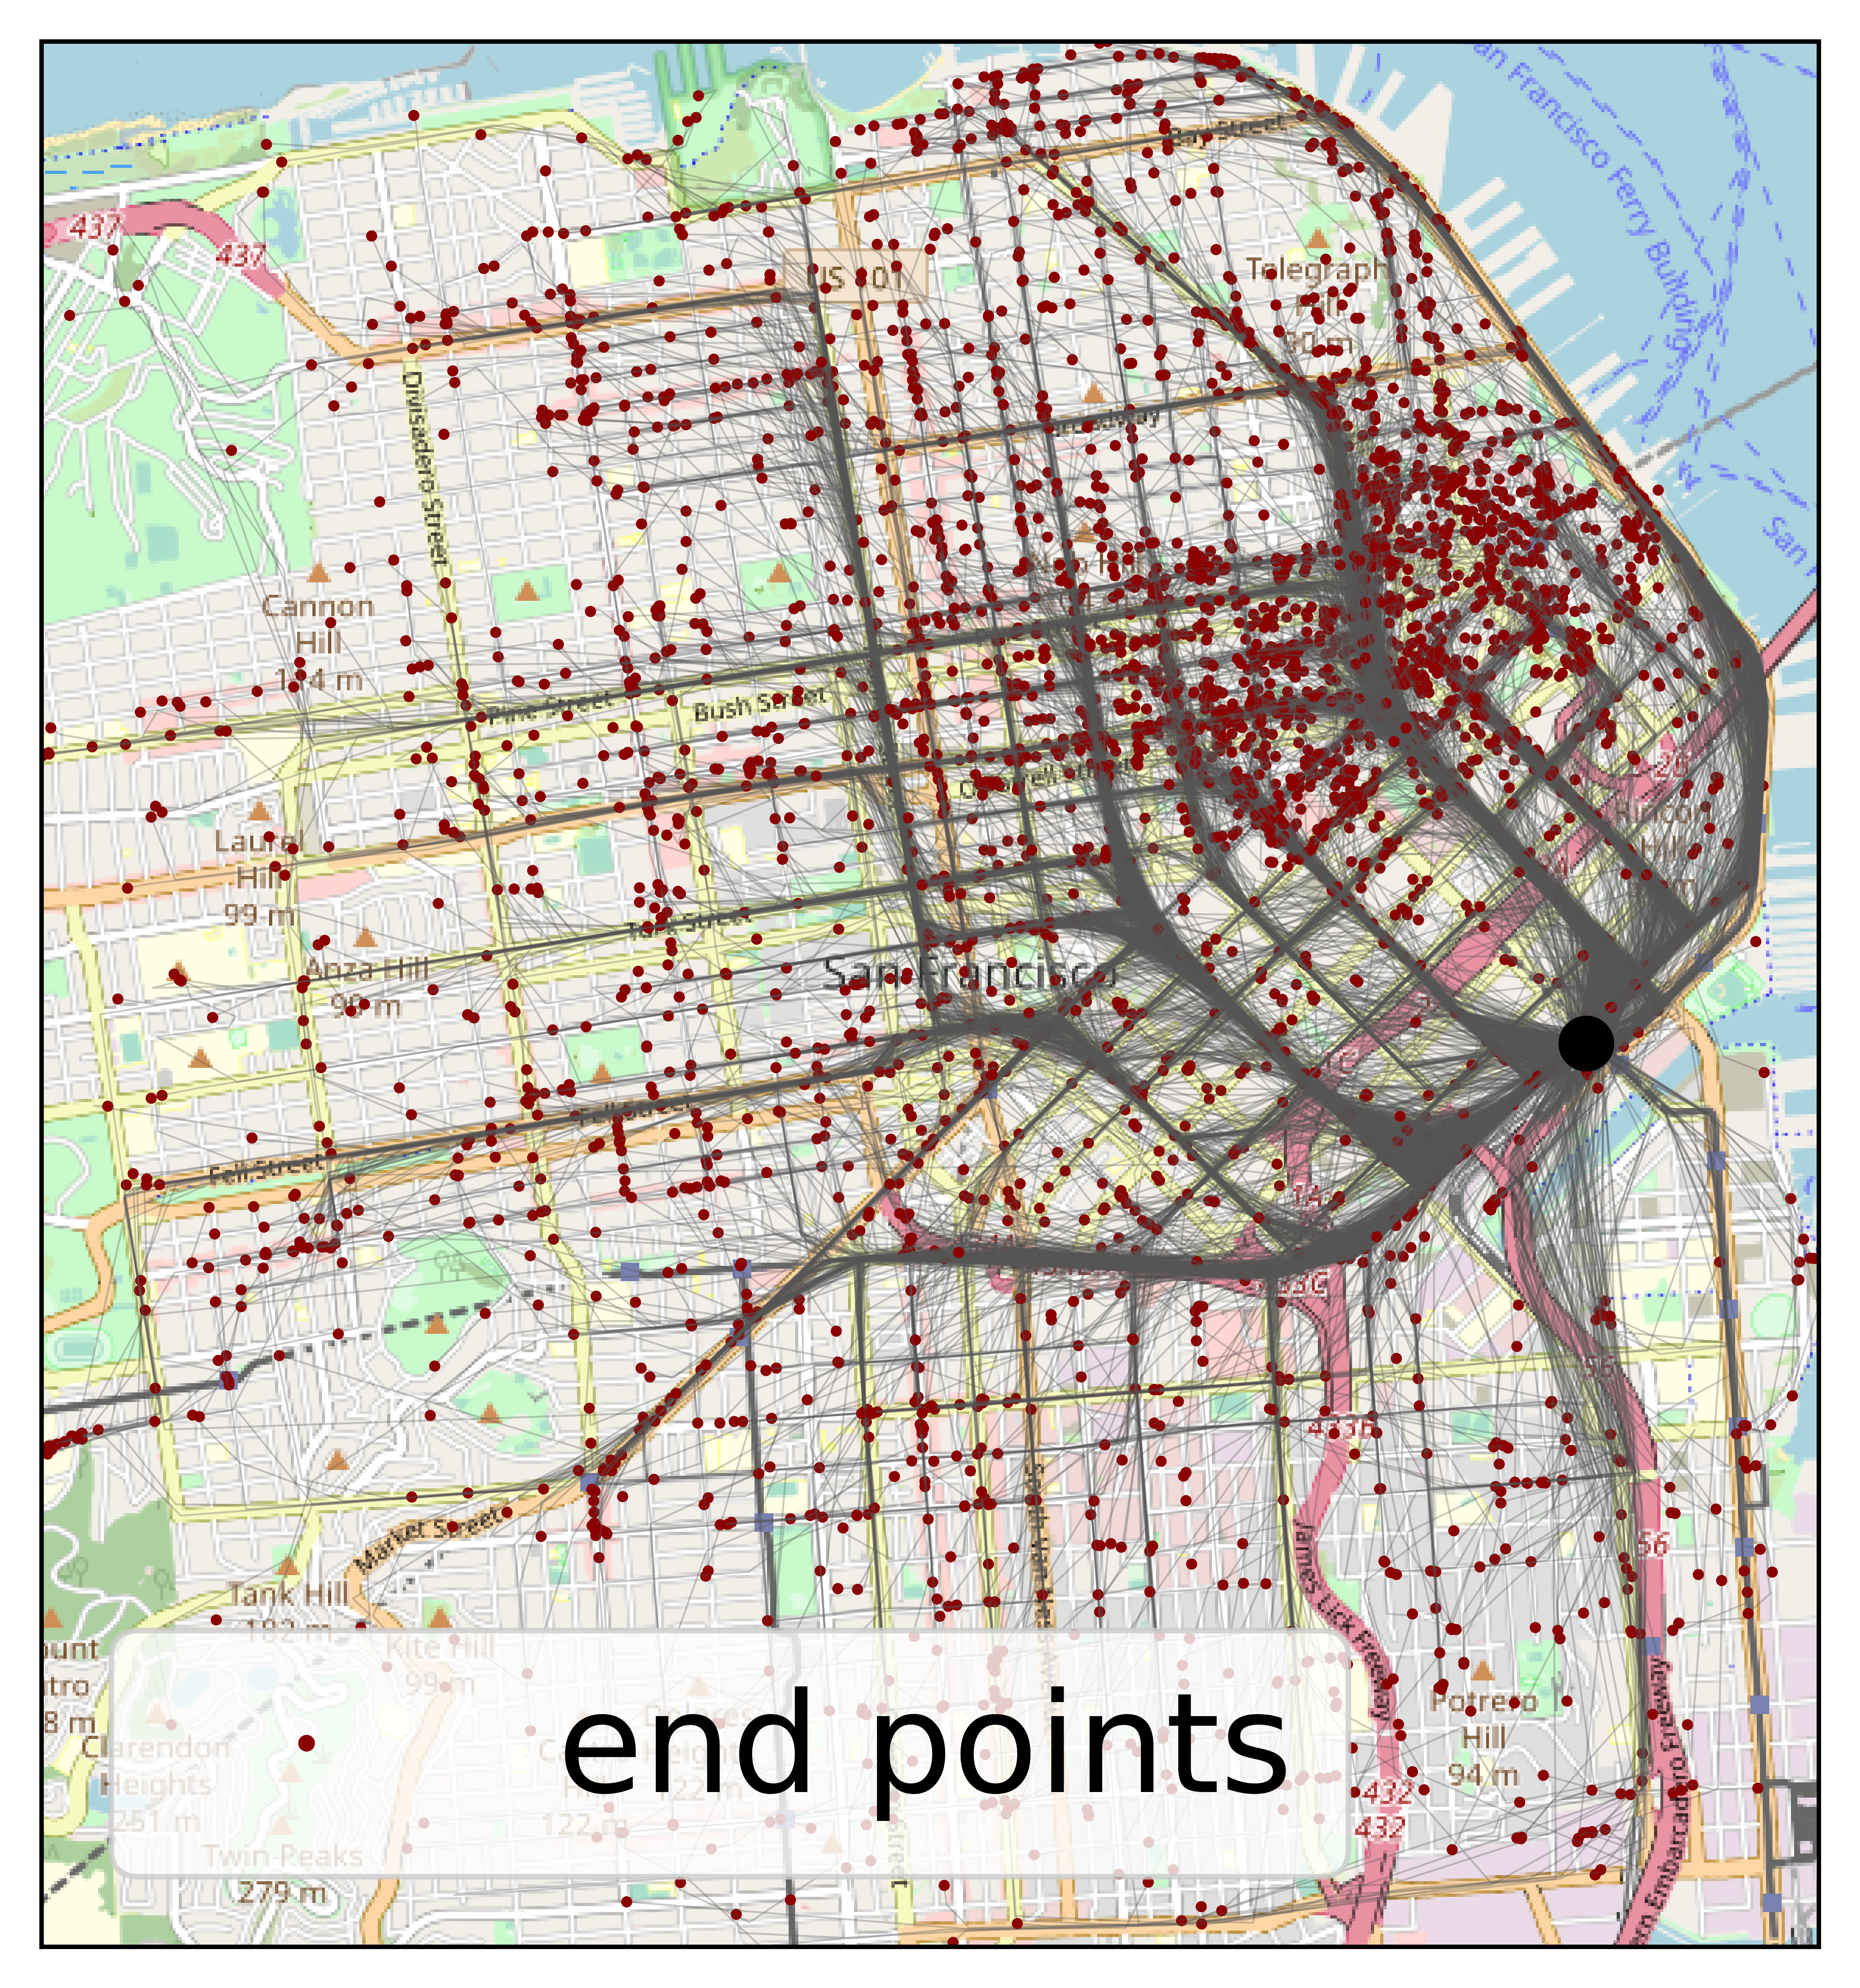
\includegraphics[width=1\textwidth]{caltrain_trajectory_map.png}
    \caption{Caltrain Trajectories Dataset}
    \label{fig37}
\end{figure}

\subsubsection{Analysis of the distances}

\begin{figure}[ht]
    \centering
    \includegraphics[width=1\textwidth]{silhouette_caltrain_score.png}
    \caption{Silhouette Score}
    \label{fig38}
\end{figure}

\autoref{fig38} hardly determine optimal number of clusters as it ranges from 10 to 15 clusters. The shape-based distances (HC-SIM, Frechet, Hausdorff) are slightly better than warping-based distances (DTW, LCSS) as the Silhouette scores are higher. We chose 15 as the number of clusters for all distances then compare the results.

\begin{tabularx}{\linewidth}{|X|X|X|X|X|X|}
    \caption{Caltrain Silhouette Scores} \\
    \hline \textbf{Clusters} & \textbf{HC-SIM} & \textbf{DTW} & \textbf{LCSS} & \textbf{Frechet} & \textbf{Hausdorff} \\
    \hline
    \hline
    2 & 0.356769 & 0.396301 & 0.285650 & 0.392788 & 0.497644 \\
    3 & 0.383545 & 0.361110 & 0.181747 & 0.347808 & 0.263201 \\
    4 & 0.349602 & 0.250431 & 0.199539 & 0.328405 & 0.225499 \\
    5 & 0.340964 & 0.262857 & 0.150745 & 0.227275 & 0.209657 \\
    6 & 0.346317 & 0.250004 & 0.143371 & 0.225573 & 0.203689 \\
    7 & 0.329542 & 0.244371 & 0.149779 & 0.254266 & 0.214275 \\
    8 & 0.330136 & 0.178117 & 0.136986 & 0.283555 & 0.202706 \\
    9 & 0.254469 & 0.180204 & 0.122737 & 0.270990 & 0.173631 \\
    10 & 0.238627 & 0.187296 & 0.106858 & 0.275026 & 0.193501 \\
    11 & 0.241977 & 0.175068 & 0.055147 & 0.241094 & 0.216469 \\
    12 & 0.236761 & 0.168340 & 0.062208 & 0.217643 & 0.213491 \\
    13 & 0.237156 & 0.162590 & 0.052939 & 0.217235 & 0.223876 \\
    14 & 0.227760 & 0.165999 & 0.046684 & 0.219286 & 0.224394 \\
    15 & 0.230400 & 0.142160 & 0.045190 & 0.214171 & 0.223323 \\
    16 & 0.222628 & 0.152119 & 0.038973 & 0.224474 & 0.219284 \\
    17 & 0.221845 & 0.153264 & 0.031790 & 0.222994 & 0.225172 \\
    18 & 0.217480 & 0.165421 & 0.033072 & 0.240360 & 0.221023 \\
    19 & 0.219536 & 0.172252 & 0.031080 & 0.239041 & 0.219824 \\
    20 & 0.214589 & 0.170462 & 0.023866 & 0.240447 & 0.216707 \\
    21 & 0.206516 & 0.164810 & 0.021384 & 0.239794 & 0.218972 \\
    22 & 0.191256 & 0.164906 & 0.019465 & 0.239200 & 0.212498 \\
    23 & 0.196210 & 0.165379 & 0.020849 & 0.244760 & 0.210494 \\
    24 & 0.200200 & 0.159268 & 0.020066 & 0.246877 & 0.203208 \\
    25 & 0.201813 & 0.159507 & 0.019265 & 0.237252 & 0.198961 \\
    26 & 0.204181 & 0.159889 & 0.019530 & 0.224376 & 0.204022 \\
    27 & 0.201373 & 0.160609 & 0.015587 & 0.222180 & 0.205813 \\
    28 & 0.201114 & 0.157332 & 0.004293 & 0.218555 & 0.202371 \\
    29 & 0.207140 & 0.156469 & 0.005048 & 0.215885 & 0.206669 \\
    30 & 0.211101 & 0.153877 & 0.005816 & 0.214025 & 0.207684 \\
    31 & 0.210175 & 0.153821 & 0.005007 & 0.211167 & 0.208809 \\
    32 & 0.205037 & 0.151434 & 0.006237 & 0.213311 & 0.208455 \\
    33 & 0.201024 & 0.122437 & 0.006821 & 0.215603 & 0.210904 \\
    34 & 0.203483 & 0.119329 & 0.004895 & 0.216018 & 0.212265 \\
    35 & 0.200473 & 0.118081 & 0.005463 & 0.217762 & 0.220704 \\
    36 & 0.202384 & 0.112060 & 0.003677 & 0.222247 & 0.223063 \\
    37 & 0.197390 & 0.111081 & 0.001623 & 0.224556 & 0.223387 \\
    38 & 0.197010 & 0.112646 & -0.001083 & 0.223489 & 0.228722 \\
    39 & 0.200355 & 0.110885 & -0.001366 & 0.226141 & 0.230493 \\
    40 & 0.201805 & 0.105598 & -0.001820 & 0.218708 & 0.236885 \\
    41 & 0.198826 & 0.106026 & -0.001056 & 0.220735 & 0.233837 \\
    42 & 0.198403 & 0.106980 & -0.011015 & 0.220628 & 0.235701 \\
    43 & 0.196807 & 0.105476 & -0.011598 & 0.218004 & 0.231970 \\
    44 & 0.189037 & 0.105457 & -0.012231 & 0.210478 & 0.227581 \\
    45 & 0.188693 & 0.105263 & -0.012043 & 0.208605 & 0.225654 \\
    46 & 0.189510 & 0.104289 & -0.011958 & 0.210598 & 0.226802 \\
    47 & 0.187696 & 0.102868 & -0.012662 & 0.208361 & 0.227238 \\
    48 & 0.188798 & 0.102793 & -0.012089 & 0.208134 & 0.229546 \\
    49 & 0.187074 & 0.103403 & -0.012561 & 0.210294 & 0.228537 \\
    50 & 0.191232 & 0.103788 & -0.014111 & 0.209117 & 0.232126 \\
    51 & 0.191061 & 0.106281 & -0.014281 & 0.207811 & 0.230924 \\
    52 & 0.188551 & 0.105691 & -0.014113 & 0.205573 & 0.229375 \\
    53 & 0.187468 & 0.105492 & -0.014115 & 0.205149 & 0.229310 \\
    54 & 0.187984 & 0.105837 & -0.015897 & 0.197593 & 0.229700 \\
    55 & 0.188822 & 0.105679 & -0.018104 & 0.195543 & 0.229799 \\
    56 & 0.189136 & 0.101598 & -0.017671 & 0.197964 & 0.225874 \\
    57 & 0.189378 & 0.100226 & -0.018083 & 0.197667 & 0.222617 \\
    58 & 0.177276 & 0.100837 & -0.017139 & 0.200659 & 0.222915 \\
    59 & 0.176738 & 0.096370 & -0.016870 & 0.201189 & 0.224060 \\
    60 & 0.177556 & 0.096224 & -0.018398 & 0.195921 & 0.226399 \\
    61 & 0.178655 & 0.093656 & -0.020441 & 0.195627 & 0.225817 \\
    62 & 0.179329 & 0.092366 & -0.022498 & 0.194352 & 0.226085 \\
    63 & 0.179318 & 0.089905 & -0.022514 & 0.196077 & 0.226631 \\
    64 & 0.179784 & 0.089470 & -0.022062 & 0.195626 & 0.224136 \\
    65 & 0.177671 & 0.089635 & -0.021617 & 0.195710 & 0.222778 \\
    66 & 0.176759 & 0.086727 & -0.022680 & 0.197178 & 0.219825 \\
    67 & 0.176586 & 0.085264 & -0.022528 & 0.197277 & 0.220204 \\
    68 & 0.177366 & 0.085366 & -0.022400 & 0.198324 & 0.220077 \\
    69 & 0.174087 & 0.085466 & -0.021788 & 0.199188 & 0.221409 \\
    70 & 0.174291 & 0.082765 & -0.022104 & 0.198879 & 0.207809 \\
    71 & 0.170972 & 0.081721 & -0.025239 & 0.199053 & 0.202763 \\
    72 & 0.170995 & 0.080905 & -0.027962 & 0.198781 & 0.202938 \\
    73 & 0.172749 & 0.080132 & -0.027751 & 0.199451 & 0.202961 \\
    74 & 0.174867 & 0.084109 & -0.029748 & 0.200830 & 0.203637 \\
    75 & 0.175850 & 0.084758 & -0.030406 & 0.198680 & 0.202993 \\
    76 & 0.174353 & 0.084321 & -0.030973 & 0.198616 & 0.205167 \\
    77 & 0.174953 & 0.085100 & -0.032215 & 0.196021 & 0.204680 \\
    78 & 0.173249 & 0.084901 & -0.031974 & 0.195357 & 0.208015 \\
    79 & 0.171855 & 0.082722 & -0.032416 & 0.192647 & 0.206051 \\
    80 & 0.167248 & 0.081761 & -0.032063 & 0.192481 & 0.207178 \\
    81 & 0.154736 & 0.082040 & -0.032430 & 0.192582 & 0.205017 \\
    82 & 0.146156 & 0.081407 & -0.032513 & 0.192138 & 0.202493 \\
    83 & 0.144325 & 0.078929 & -0.032250 & 0.193020 & 0.200483 \\
    84 & 0.144089 & 0.077166 & -0.032722 & 0.196295 & 0.200646 \\
    85 & 0.142328 & 0.077269 & -0.033828 & 0.194151 & 0.200086 \\
    86 & 0.141368 & 0.075914 & -0.035315 & 0.195398 & 0.200021 \\
    87 & 0.142270 & 0.075813 & -0.035765 & 0.196780 & 0.200021 \\
    88 & 0.142786 & 0.075910 & -0.036718 & 0.197130 & 0.202505 \\
    89 & 0.139398 & 0.076090 & -0.038886 & 0.198587 & 0.202735 \\
    90 & 0.140799 & 0.077447 & -0.038330 & 0.196552 & 0.204501 \\
    91 & 0.140396 & 0.077685 & -0.038376 & 0.195879 & 0.203706 \\
    92 & 0.140974 & 0.076298 & -0.040412 & 0.192209 & 0.203204 \\
    93 & 0.141698 & 0.076249 & -0.040812 & 0.195462 & 0.204461 \\
    94 & 0.141920 & 0.075422 & -0.041572 & 0.196538 & 0.205025 \\
    95 & 0.140590 & 0.075472 & -0.041368 & 0.198024 & 0.204963 \\
    96 & 0.139228 & 0.074794 & -0.041593 & 0.198072 & 0.207391 \\
    97 & 0.139199 & 0.073772 & -0.041751 & 0.195956 & 0.206780 \\
    98 & 0.139347 & 0.072257 & -0.041865 & 0.199066 & 0.207357 \\
    99 & 0.139909 & 0.072388 & -0.041977 & 0.197660 & 0.206953 \\
    100 & 0.140607 & 0.072018 & -0.041886 & 0.196479 & 0.206427 
    \label{table:caltrain_silhouette}
\end{tabularx}

\autoref{fig39} illustrates visual results for all distances with 15 clusters. Based on Mopsi experiment, HC-SIM is expected to be the best. We observe that trajectories are well classified by HC-SIM according to their paths in \ref{fig44}. The clusters using HC-SIM seem to be consistent as the trajectories in each cluster grouped better than other distances. For example, the DTW cluster 5 in \autoref{fig40}, the LCSS cluster 8 in \autoref{fig41}, the Hausdorff cluster 3 in \autoref{fig42}, and the Frechet cluster 9 in \autoref{fig43} got a lot of noise.

\begin{figure}[htbp!]
    \centering
    \includegraphics[width=1\textwidth]{Caltrain Plots.png}
    \caption{Caltrain Clusters}
    \label{fig39}
\end{figure}

\begin{figure}[htbp!]
    \centering
    \includegraphics[width=1\textwidth]{Caltrain DTW.png}
    \caption{Caltrain DTW Clusters}
    \label{fig40}
\end{figure}

\begin{figure}[htbp!]
    \centering
    \includegraphics[width=1\textwidth]{Caltrain LCSS.png}
    \caption{Caltrain LCSS Clusters}
    \label{fig41}
\end{figure}

\begin{figure}[htbp!]
    \centering
    \includegraphics[width=1\textwidth]{Caltrain Hausdorff.png}
    \caption{Caltrain Hausdorff Clusters}
    \label{fig42}
\end{figure}

\begin{figure}[htbp!]
    \centering
    \includegraphics[width=1\textwidth]{Caltrain Frechet.png}
    \caption{Caltrain Frechet Clusters}
    \label{fig43}
\end{figure}

\begin{figure}[htbp!]
    \centering
    \includegraphics[width=1\textwidth]{Caltrain HCSIM.png}
    \caption{Caltrain HC-SIM Clusters}
    \label{fig44}
\end{figure}

\pagebreak

\section{Conclustions}
Clustering trajectories is heavily dependent on the selection of an appropriate distance. In this thesis, we explored several distances concentrating on various characteristics of trajectories. All distances seem to work well with the hierarchical agglomerative clustering (HAC) method to cluster trajectories. Based on our experiment, shape-based distances give better clusters than warping-base ones, especially HC-SIM enables us obtain good clusters that nearly match ground-truth data. Both clustering and validation methods that we use in this thesis work well and give good results. This may be used to address a variety of problems. From learning moving objects' behavior, many applications are able to recommend locations to visit or arrange a city's trip based on that result.

\pagebreak

% Two common styles, pick one or find alternate bst.
% \citet{john} is like John (1985); \citep{jane} is like (Jane 1985)
%\bibliographystyle{IEEEtranN} % Like this (Jane 1995)
\bibliographystyle{apacite} % Like this [6] 
\bibliography{thesis}

\end{document}